\documentclass[11pt, a4paper, oneside]{book}
\usepackage{amsmath, amsthm, amssymb, bm, graphicx, hyperref, mathrsfs}

%%%%%%%% CREATE DOCUMENT STRUCTURE %%%%%%%%
%% Language and font encodings
\usepackage[english]{babel}
\usepackage[utf8x]{inputenc}
\usepackage[T1]{fontenc}
%\usepackage{subfig}

%% Sets page size and margins
\usepackage[a4paper,top=2cm,bottom=2.5cm,left=1.5cm,right=1.5cm,marginparwidth=1.75cm]{geometry}

%user package
\usepackage{setspace}
\usepackage{enumitem}
\usepackage{float}
\usepackage{subfigure}
% \usepackage{indentfirst}

% 首行缩进
% \setlength{\parindent}{2em}

\title{{\Huge{\textbf{Cryptography and Security}}}\\}
\author{Jiaxuan Zhang}
\date{\today}
\linespread{1.2}
\newtheorem{theorem}{Theorem}[section]
\newtheorem{definition}[theorem]{Definition}
\newtheorem{lemma}[theorem]{Lemma}
\newtheorem{corollary}[theorem]{Corollary}
\newtheorem{example}[theorem]{Example}
\newtheorem{proposition}[theorem]{Proposition}
\newtheorem{model}[theorem]{Model}
\newtheorem{method}[theorem]{Method}

\begin{document}

\maketitle
\pagenumbering{roman}
\setcounter{page}{1}

\begin{center}
    \Huge\textbf{Forword}
\end{center}

\begin{flushright}
    \begin{tabular}{c}
        Jiaxuan Zhang\\
        \today
    \end{tabular}
\end{flushright}

\newpage
\pagenumbering{Roman}
\setcounter{page}{1}
\tableofcontents
\newpage
\setcounter{page}{1}
\pagenumbering{arabic}


\part{Coursera Stanford Cryptography I}

\chapter{Introduction}



\section{Goals of Crypto}

\subsubsection{Confidentality}

\subsubsection{Integrity}
we make sure that the received message is equal to the sent one


\subsubsection{Authenticated}
we make sure about who sent the message

\section{Some Historic Examples}

\subsection{Substitution Cipher: Caesar Cipher}


\subsubsection{How to break a substitution cipher}

\begin{enumerate}
    \item use frequency of English letters
    \item use frequency of pairs of letters
\end{enumerate}


\subsection{Vigener Cipher}

The format of Vigener Cipher is shown in Figure \ref{fig: 01 Vigener Cipher}.

\begin{figure}
    \centering
    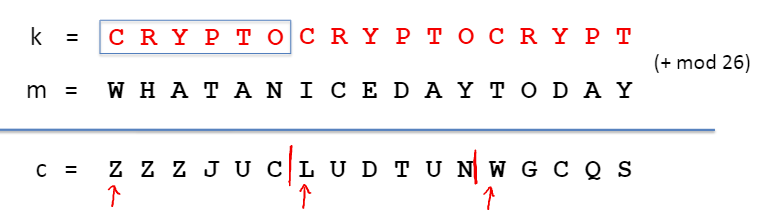
\includegraphics[width=0.8\textwidth]{Stanford_Crypto_1/fig/01_Introduction/Vigener Cipher.png}
    \caption{Vigener Cipher}
    \label{fig: 01 Vigener Cipher}
\end{figure}


\section{Introduction of Discrete Probability}


\subsection{Randomized Algorithms}

\subsubsection{Deterministic Algorithm}

$$y \leftarrow A(m)$$. 

\subsubsection{Randomized Algorithm}

$$
y \longleftarrow A(m ; r) \quad \text { where } \quad r \longleftarrow\{0,1\}^{n}
$$

So the output of $A(m)$ is a random variable

$$
\mathrm{y} \leftrightarrow \mathrm{A}(\mathrm{m})
$$



\subsection{An Important Property of XOR}

\begin{theorem} [An Important Property of XOR]  An Important Property of XOR:
    $Y$ a \textbf{rand. var.} over $\{0,1\}^{n}, \quad X$ an \textbf{indep. uniform var.} on $\{0,1\}^{n}$
    Then $Z:=Y \oplus X$ is uniform var. on $\{0,1\}^{n}$
    
\end{theorem}


\subsection{The Birthday Paradox}

\begin{theorem} [The Birthday Paradox] The Birthday Paradox:

    Let $r_{1}, \ldots, r_{n} \in U \quad$ be indep. identically distributed random vars.
    when $\mathrm{n}=1.2 \times|\mathrm{U}|^{1 / 2}$ then $\operatorname{Pr}\left[\exists \mathrm{i} \neq \mathrm{j}: r_{\mathrm{i}}=r_{\mathrm{j}}\right] \geq 1 / 2$
    
\end{theorem}

\section{Semantic Security}

Here, we summarized different Semantic Security Models and Definitions.

\chapter{Stream Cipher}
\section{Information Theoretic Security and The One Time Pad}

\subsection{Symmetric Ciphers}

\begin{definition} [Symmetric Cipher] Symmetric Cipher

    Aa cipher defined over $(\mathcal{K}, M, 6) \quad(k, M, c)$ is a pair of "efficient" algs $(\boldsymbol{E}, \boldsymbol{D})$ where 
    $E: \mathcal{K} \times M \rightarrow 6$,  $D: \mathcal{K} \times C \rightarrow \mu$
    s.t. $\forall m \in M, k \in \mathscr{L}: \quad D(k, E(k, m))=m$
    
\end{definition}

\textbf{Notes:}
\begin{itemize} [itemsep=2pt,topsep=0pt,parsep=0pt]
    \item efficient means: can be calculated in a certain polynomial time limit
    \item $E$ is often Randomized
    \item $D$ is always deterministic
\end{itemize}

\subsection{Perfect Security}

\begin{definition} [Shannon Information Theoretic Security] Shannon Information Theoretic Security:

    A cipher $(E, D)$ over $(K, M, C)$ has perfect secrecy if
    $\forall m_{0}, m_{1} \in M \quad\left(\left|m_{0}\right|=\left|m_{1}\right|\right)$ and $\forall c \in C$
    $\operatorname{Pr}\left[E\left(k, m_{0}\right)=c\right]=\operatorname{Pr}\left[E\left(k, m_{1}\right)=c\right]$ where $k \leftarrow^{R} k$
    
\end{definition}

\textbf{Notes: }
\begin{itemize} [itemsep=2pt,topsep=0pt,parsep=0pt]
    \item Given CT, adv. cannot tell if message is $m_0$ or $m_1$
    \item most powerful adv. learns nothing about PT from CT
\end{itemize}


\begin{theorem}
    perfect security $\Rightarrow$ $\mathcal{K} \ge \mathcal{M}$.
\end{theorem}


\subsection{The One-Time Pad: Vernam Cipher}

\begin{definition} [One-Time Pad]

    A one-time pad is a symmetric cipher $\mathcal{E}=(E, D)$, where the keys, messages, and ciphertexts are bit strings of the same length; that is, $\mathcal{E}$ is defined over $(\mathcal{K}, \mathcal{M}, \mathcal{C})$, where
    $$
    \mathcal{K}:=\mathcal{M}:=\mathcal{C}:=\{0,1\}^{L}
    $$
    for some fixed parameter $L$. For a key $k \in\{0,1\}^{L}$ and a message $m \in\{0,1\}^{L}$ the encryption function is defined as follows:
    $$
    E(k, m):=k \oplus m,
    $$
    and for a key $k \in\{0,1\}^{L}$ and ciphertext $c \in\{0,1\}^{L}$, the decryption function is defined as follows:
    $$
    D(k, c):=k \oplus c .
    $$
    
\end{definition}


\begin{theorem} [Inf Secure of OTP] Inf Secure of OTP:

    OTP has perfect security.
    
\end{theorem}


\section{Pseudo Random Generators}


\begin{definition} [Pseudo Random Generators] Pseudo Random Generators:
    $P R G$ is a function $G: \underbrace{\{0,1\}^{s}}_{\text {seed } \atop \text { space }} \rightarrow\{0,1\}^{n} \quad n \gg s$
    (eff. computable by deterministic algorithn )
\end{definition}

\subsection{Security of RPG}

\begin{definition} [negligible and non-negligible] negligible and non-negligible

    $$
    \varepsilon \text { is a function } \varepsilon: \mathbf{Z}^{20} \rightarrow \mathbf{R}^{20} \text { and }
    $$

    $$
    \begin{array}{ll}
    \varepsilon \text { non-neg: } \quad \exists d: \varepsilon(\lambda) \geq 1 / \lambda^{d} \text { inf. often } & (\varepsilon \geq 1 / \text { poly, for many } \lambda) \\
    \varepsilon \text { negligible: } \forall d, \lambda \geq \lambda_{d}: \quad \varepsilon(\lambda) \leq 1 / \lambda^{d} & (\varepsilon \leq 1 / \text { poly, for large } \lambda)
    \end{array}
    $$
        
    
\end{definition}

\begin{method} [Attack Game of Unpred. PRG] Attack Game of Unpred. PRG

    Attack Game 3.2 (Unpredictable $\boldsymbol{P R G}$ ). For a given PRG $G$, defined over $\left(\mathcal{S},\{0,1\}^{L}\right)$, and a given adversary $\mathcal{A}$, the attack game proceeds as follows:
    \begin{enumerate} [itemsep=2pt,topsep=0pt,parsep=0pt]
        \item The adversary sends an index $i$, with $0 \leq i \leq L-1$, to the challenger.
        \item The challenger computes
        $$
        s \stackrel{\mathrm{R}}{\mathcal{S}}, r \leftarrow G(s)
        $$
        \item he adversary outputs $g \in\{0,1\}$.
    \end{enumerate}
    We say that $\mathcal{A}$ wins if $r[i]=g$, and we define $\mathcal{A}$ 's advantage $\operatorname{Predadv}[\mathcal{A}, G]$ to be $\mid \operatorname{Pr}[\mathcal{A}$ wins $]-1 / 2 \mid$.
    
\end{method}

\begin{definition} [Unpredictable PRG] Unpredictable PRG
    A PRG G is unpredictable if the value Predadv[A, G] is negligible for all efficient adversaries A.
\end{definition}

\textbf{Notes: When implementation, never use} \verb!random()! \textbf{for crypto!}

\begin{method} [Attack Game of PRG] Attack Game of PRG
    Attack Game $3.1(P R G)$. For a given PRG $G$, defined over $(\mathcal{S}, \mathcal{R})$, and for a given adversary $\mathcal{A}$, we define two experiments, Experiment 0 and Experiment 1 . For $b=0,1$, we define:
    Experiment $b$ :
    - The challenger computes $r \in \mathcal{R}$ as follows:
    if $b=0: s \longleftarrow \mathcal{R}, r \leftarrow G(s) ;$
    if $b=1: r \longleftarrow{R} \mathcal{R}$.

\end{method}

\begin{definition} [Secure PRG] Secure PRG:

    For $b=0,1$, let $W_{b}$ be the event that $\mathcal{A}$ outputs 1 in Fixperiment $b$. We define $\mathcal{A}$ 's advantage with respect to $G$ as
    $$
    \operatorname{PRGadv}[\mathcal{A}, G]:=\left|\operatorname{Pr}\left[W_{0}\right]-\operatorname{Pr}\left[W_{1}\right]\right|
    $$
    A $P R G G$ is secure if the value $\operatorname{PRGadv}[\mathcal{A}, G]$ is negligible for all efficient adversaries $\mathcal{A}$.
    
\end{definition}

\begin{theorem} [Unpredictable and Secure PRG]

    if $\forall i \in \{0,\cdots,n-1\}$ PRG G is unpredictable at pos. i, then G is a secure PRG.
    
\end{theorem}

\textbf{Notes:} A secure PRG is unpredictable. if next-bit predictors cannot distinguish G from random then no statistical test can


\section{Stream Ciphers: Encrpytion with a PRG}

Idea:  replace "random" key by "pseudorandom" key.

\begin{method} [Stream Cipher] Stream Cipher

    Making OTP practical using a PRG:
    G: $\mathrm{K} \longrightarrow\{0,1\}^{\mathrm{n}}$
    Stream cipher:
    $\mathrm{E}(\mathrm{k}, \mathrm{m})=\mathrm{m} \bigoplus \mathrm{G}(\mathrm{k}) \quad, \quad \mathrm{D}(\mathrm{k}, \mathrm{c})=\mathrm{c} \bigoplus \mathrm{G}(\mathrm{k})$

\end{method}

\section{Attacks on Stream Ciphers and The One Time Pad}

\subsubsection{Two-Time Pad is Insecure}

$$
\begin{aligned}
&c_{1} \leftarrow m_{1} \oplus P R G(k) \\
&c_{2} \leftarrow m_{2} \oplus P R G(k)
\end{aligned}
$$
Eavesdropper does:
$$
\mathrm{C}_{1} \oplus \mathrm{C}_{2} \rightarrow m_{1} \oplus \mathrm{m}_{2}
$$


\textbf{Notes: Never use stream cipher key more than once!}
\begin{itemize} [itemsep=2pt,topsep=0pt,parsep=0pt]
    \item Network traffic: negotiate new key for every session
    \item Disk encryption: typically do not use a stream cipher
\end{itemize}


\subsubsection{One-Time Pad is malleable: not integrity}

Modifications to ciphertext are undetected and  have predictable impact on plaintext

\section{Real-World Stream Ciphers}

\subsection{Old Example: CSS}

The process of CSS is shown in Figure \ref{fig: 02 CSS}.

\begin{figure}[h]
    \centering
    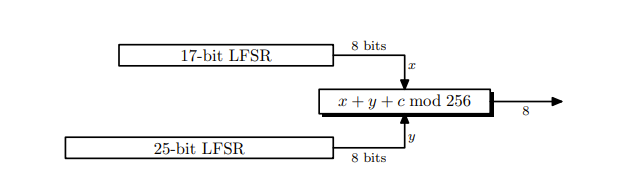
\includegraphics[width=0.8\textwidth]{Stanford_Crypto_1/fig/02_Stream_Cipher/CSS Stream Cipher.png}
    \caption{CSS}
    \label{fig: 02 CSS}
\end{figure}

\subsubsection{Linear feedback shift registers (LFSR)}

The LFSR is a key structure in CSS. The structure of LFSR is shown in Figure \ref{fig: 02 LFSR}.

\begin{figure}[h]
    \centering
    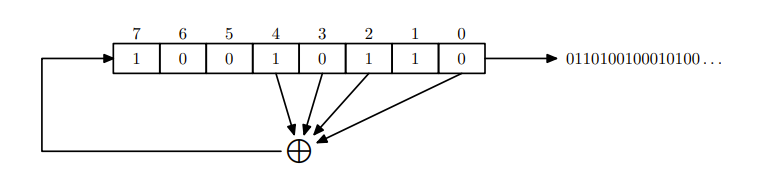
\includegraphics[width=0.8\textwidth]{Stanford_Crypto_1/fig/02_Stream_Cipher/LFSR.png}
    \caption{LFSR}
    \label{fig: 02 LFSR}
\end{figure}


\subsection{Modern Example: eStream: Salsa20}

\subsubsection{eStream Framework}

PRG: $\underbrace{\{0,1\}^{s}}_{\text {seed }} \times R \rightarrow\{0,1\}^{n} \quad n>>s$

\textbf{Nonce}: a non-repeating value for a given key. $R$ is Nonce

$\mathrm{E}(\mathrm{k}, \mathrm{m} ; \mathrm{r})=\mathrm{m} \bigoplus \mathrm{PRG}(\mathrm{k} ; \mathrm{r})$

The pair $(k, r)$ is never used more than once.


\subsubsection{Salsa20}

\begin{equation}
    \begin{aligned}
        &\text { Salsa20: }\{0,1\}^{128 \text { or } 256} \times\{0,1\}^{64} \longrightarrow\{0,1\}^{\mathrm{n}} \quad\left(\max \mathrm{n}=2^{73}\right. \text { bits) } \\
        &\text { Salsa20 }(\mathrm{k} ; \mathrm{r}):=\mathrm{H}(\mathrm{k},(\mathrm{r}, 0))\|\mathrm{H}(\mathrm{k},(\mathrm{r}, 1))\| \ldots
    \end{aligned}
\end{equation}

The structure of Salsa20 is shown in Figure \ref{fig: 02 Salsa20}.

\begin{figure}
    \centering
    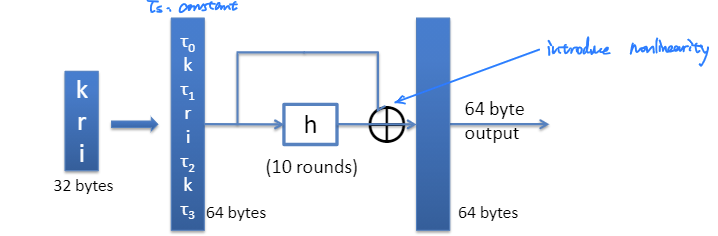
\includegraphics[width=0.6\textwidth]{Stanford_Crypto_1/fig/02_Stream_Cipher/Salsa20.png}
    \caption{Salsa20}
    \label{fig: 02 Salsa20}
\end{figure}

\section{Security Analysis of Stream Ciphers}

\subsection{Semantic Security for One-Time Pad}

\begin{method} [Attack Game for Semantic Security] Attack Game for Semantic Security

    For   $b=0,1$   define experiments EXP(0) and EXP(1) as

    \begin{enumerate} [itemsep=2pt,topsep=0pt,parsep=0pt]
        \item The adversary computes $m0, m1 \in M$, of the same length, and sends them to the challenger.
        \item The challenger computes $k \leftarrow^R K$, $c \leftarrow^R E(k, mb)$, and sends $c$ to the adversary.
        \item The adversary outputs a bit $\hat{b} \in \{0, 1\}$.
    \end{enumerate}


\end{method}



\begin{definition} [Semantic Security] Semantic Security

    For $b=0,1$, let $W_{b}$ be the event that $\mathcal{A}$ outputs 1 in Experiment $b$. We define $\mathcal{A}$ 's semantic security advantage with respect to $\mathcal{E}$ as
    $$
    \operatorname{SSadv}[\mathcal{A}, E]:=\left|\operatorname{Pr}\left[W_{0}\right]-\operatorname{Pr}\left[W_{1}\right]\right|
    $$

    A cipher E is semantically secure if for all efficient adversaries A, the value $SSadv[A, E$] is negligible
    
\end{definition}


\subsection{Stream Ciphers are Semantically Secure}

\begin{theorem} [OPT Sem. Sec.] OPT Sem. Sec.

    OTP is semantically secure
    
\end{theorem}


\section{Summary}

Starting from OTP and the theorem of \textbf{Perfect Security}, we point out the the OTP met the Confidentiality as long as the key length is equal to message length. But it is impossible in practice.

Stream cipher tries to solve this problem by using a key to generate a series of pseudorandom keys. In order to do that, we need to guarantee the process of generate a pseudorandom keys do not harm the security.

So we define what is a secure PRG and relate it with unpredictable. We can also prove that the OTP is Sem. secure with a secure RPG.

\chapter{Block Cipher}


\section{PRPs and PRFs}

\begin{definition} [PRP] PRP: 

    Pseudo Random Permutation (PRP) defined over (K,X):
    $\mathrm{E}: \mathrm{K} \times \mathrm{X} \rightarrow \mathrm{X}$
    such that:
    \begin{enumerate} [itemsep=2pt,topsep=0pt,parsep=0pt]
        \item Exists "efficient" deterministic algorithm to evaluate $E(k, x)$
        \item The function $E(k, \cdot)$ is one-to-one
        \item Exists "efficient" inversion algorithm $D(k, y)$
    \end{enumerate}
    
\end{definition}


\begin{definition} [PRF] PRF:

    Pseudo Random Function (PRF) defined over (K,X,Y):
    $F: K \times X \rightarrow Y \rightarrow$ 
    such that exists "efficient" algorithm to evaluate $F(k, x)$

\end{definition}

\subsection{Secure PRFs and Secure PRPs}

From intuition, a PRF is secure if a random function in $Funs[X,Y]$ is indistinguishable from a random function in $S_F$. The experiment for secure PRF is shown in Figure \ref{fig: 03 Secure PRF Experiment}.

\begin{figure}[h]
    \centering
    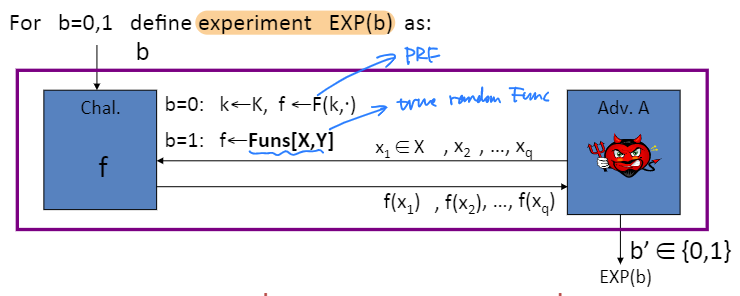
\includegraphics[width=0.5\textwidth]{Stanford_Crypto_1/fig/03_block_cipher/Secure PRF Experiment.png}
    \caption{Secure PRF Experiment}
    \label{fig: 03 Secure PRF Experiment}
\end{figure}

\begin{definition} [Secure PRF] Secure PRF

    $F$ is a secure PRF if for all "efficient" A:
    $$
    \operatorname{Adv}_{\mathrm{PRF}}[A, \mathrm{~F}]:=|\operatorname{Pr}[\operatorname{EXP}(0)=1]-\operatorname{Pr}[\operatorname{EXP}(1)=1]|
    $$
    is "negligible."
    
\end{definition}

The experiment for secure PRF is shown in Figure \ref{fig: 03 Secure PRP Experiment}.

\begin{figure}[h]
    \centering
    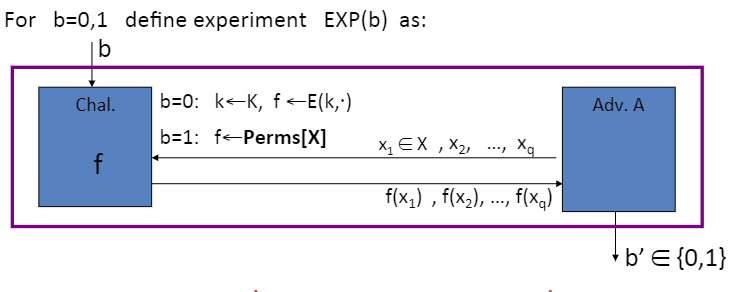
\includegraphics[width=0.5\textwidth]{Stanford_Crypto_1/fig/03_block_cipher/Secure PRP Experiment.png}
    \caption{Secure PRP Experiment}
    \label{fig: 03 Secure PRP Experiment}
\end{figure}

\begin{definition} [Secure PRP] Secure PRP:

    $E$ is a secure PRP if for all "efficient" A:
    $$
    \operatorname{Adv}_{\mathrm{PRP}}[A, E]=|\operatorname{Pr}[\operatorname{EXP}(0)=1]-\operatorname{Pr}[\operatorname{EXP}(1)=1]|
    $$
    is "negligible."
    
\end{definition}

AES, 3DES are PRPs that is believed to be secure.

There is a Lemma about the relation between secure PRP and secure PRF. The lemma tell us that "any secure PRP is also a secure PRF, if $|X|$ is sufficiently large"
 
\begin{lemma} [PRF Switching Lemma] PRF Switching Lemma
    Let $\mathrm{E}$ be a PRP over $(\mathrm{K}, \mathrm{X})$
    Then for any q-query adversary A:
    $$
    \left|\operatorname{Adv}_{\text {PRF }}[A, E]-\operatorname{Adv}_{\text {PRP }}[A, E]\right|<q^{2} / 2|X|
    $$
\end{lemma}


\subsection{Constructing PRGs from PRFs}

\begin{method} [From PRFs to PRGs: 1] From PRFs to PRGs:

    Let $\mathrm{F}: \mathrm{K} \times\{0,1\}^{\mathrm{n}} \rightarrow\{0,1\}^{\mathrm{n}}$ be a secure PRF.
    Then the following $G: K \rightarrow\{0,1\}^{n t} \quad$ is a secure PRG:
    $$
    \mathrm{G}(\mathrm{k})=\mathrm{F}(\mathrm{k}, 0)\|\mathrm{F}(\mathrm{k}, 1)\| \cdots \| \mathrm{F}(\mathrm{k}, \mathrm{t}-1)
    $$
        
\end{method}

One advantage of this method is it is parallelizable.

\subsection{Constructing PRFs from PRGs}

The first method is Tree Construction that helps us generate PRFs from PRGs, the structure of the Tree Construction is shown in Figure \ref{fig: 03 Tree Construction}.

\begin{figure}[h]
    \centering
    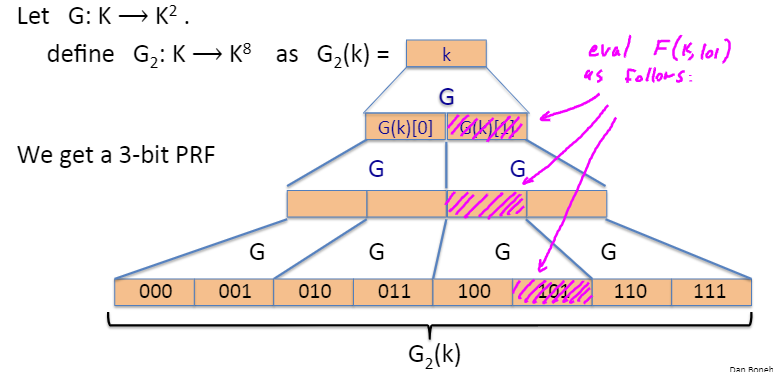
\includegraphics[width=0.5\textwidth]{Stanford_Crypto_1/fig/03_block_cipher/Tree Construction.png}
    \caption{Tree Construction}
    \label{fig: 03 Tree Construction}
\end{figure}

Another method to generate PRFs to PRGs is the GGM PRF method. Which is shown in Figure \ref{fig: 03 GGM PRF}.

\begin{figure}[h]
    \centering
    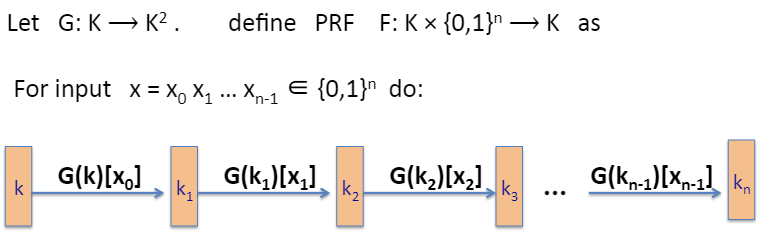
\includegraphics[width=0.5\textwidth]{Stanford_Crypto_1/fig/03_block_cipher/GGM PRF.png}
    \caption{GGM PRF}
    \label{fig: 03 GGM PRF}
\end{figure}

However, this method is quite slow, so it is not used in practice.

A property exists for these two methods: \textbf{If G is a secure PRG then the F is a secure PRF}


\section{Block Ciphers}

The structure of the block cipher is shown in Figure \ref{fig: 03 Block Cipher}.

\begin{figure}[h]
    \centering
    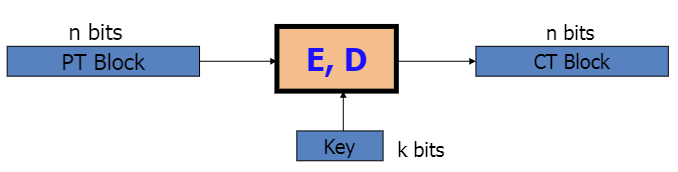
\includegraphics[width=0.8\textwidth]{Stanford_Crypto_1/fig/03_block_cipher/Block Cipher.png}
    \caption{Block Cipher}
    \label{fig: 03 Block Cipher}
\end{figure}

The general framework of the block cipher is shown in Figure \ref{fig: 03 Block Cipher Structure}

\begin{figure}[h]
    \centering
    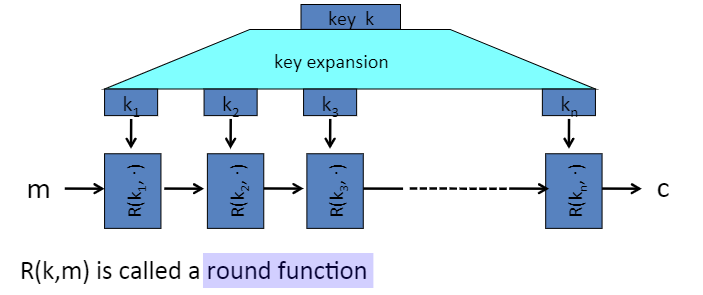
\includegraphics[width=0.8\textwidth]{Stanford_Crypto_1/fig/03_block_cipher/Block Cipher Structure.png}
    \caption{Block Cipher Structure}
    \label{fig: 03 Block Cipher Structure}
\end{figure}

\subsection{The Data Encryption Standard (DES)}

    The DES encryption algorithm is a \textbf{16-round Feistel network} where each round uses a different function $f: \mathcal{X} \rightarrow \mathcal{X}$(round function).

\subsubsection{Feistel Network}

The encryption process of Feistel Network is shown in Figure \ref{fig: 03 Feistel Network Encryption}.

\begin{figure}[h]
    \centering
    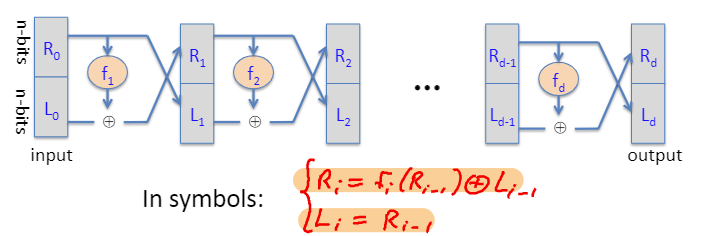
\includegraphics[width=0.8\textwidth]{Stanford_Crypto_1/fig/03_block_cipher/Feistel Network Encryption.png}
    \caption{Feistel Network Encryption}
    \label{fig: 03 Feistel Network Encryption}
\end{figure}


The decryption process of Feistel Network is shown in Figure \ref{fig: 03 Feistel Network Decryption}.

\begin{figure}[h]
    \centering
    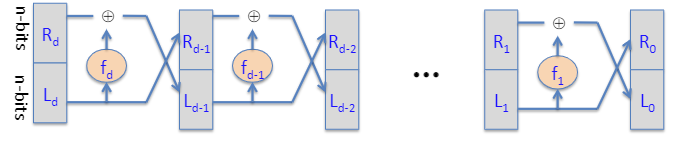
\includegraphics[width=0.8\textwidth]{Stanford_Crypto_1/fig/03_block_cipher/Feistel Network Decryption.png}
    \caption{Feistel Network Decryption}
    \label{fig: 03 Feistel Network Decryption}
\end{figure}

The inversion part is basically the same circuit with $f_1 , \cdots f_d$ applied in reverse order.

\begin{theorem} [Theorem about Security of Feistel Network] Theorem about Security of Feistel Network:

    f: $\mathrm{K} \times\{0,1\}^{\mathrm{n}} \rightarrow\{0,1\}^{\mathrm{n}}$ a secure PRF
    $\Rightarrow$ 3-round Feistel $\mathrm{F}: \mathrm{K}^{3} \times\{0,1\}^{2 \mathrm{n}} \rightarrow\{0,1\}^{2 \mathrm{n}}$ a secure PRP
    
\end{theorem}

\subsection{DES Round Function}

In round number $i$ the function $f$ is defined as
$$
f(x):=F\left(k_{i}, x\right)
$$
where $k_{i}$ is a 48 -bit key for round number $i$ and $F$ is a fixed function called the DES round function. The function $F$ is the centerpiece of the DES algorithm and is shown in Figure \ref{fig: 03 DES Round Function}.

\begin{figure}[h]
    \centering
    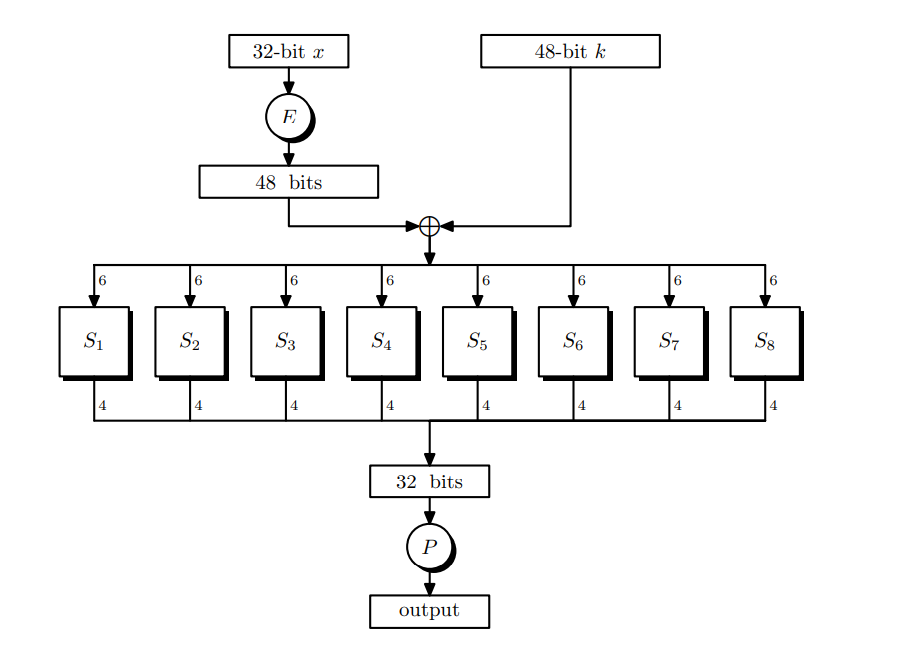
\includegraphics[width=0.8\textwidth]{Stanford_Crypto_1/fig/03_block_cipher/DES Round Function.png}
    \caption{DES Round Function}
    \label{fig: 03 DES Round Function}
\end{figure}

The auxiliary functions in the round function is shown as follows

\begin{enumerate} [itemsep=2pt,topsep=0pt,parsep=0pt]
    \item The function $E$ expands a 32-bit input to a 48-bit output by rearranging and replicating the input bits. For example, $E$ maps input bit number 1 to output bits 2 and 48 ; it maps input bit 2 to output bit number 3 , and so on.
    \item The function $P$, called the mixing permutation, maps a 32 -bit input to a 32 -bit output by rearranging the bits of the input. For example, $P$ maps input bit number 1 to output bit number 9 ; input bit number 2 to output number 15 , and so on.
    \item At the heart of the DES algorithm are the functions $S_{1}, \ldots, S_{8}$ called S-boxes. Each S-box $S_{i}$ maps a 6-bit input to a 4-bit output by a lookup table. The DES standard lists these 8 look-up tables, where each table contains 64 entries.
\end{enumerate}

It is important to choose appropriate S-BOXES and P-BOXES.

\subsubsection{Triple DES}

For Normal DES with a 56-bit cipher, it can be broken in 7 days. So we need more method to make DES more safety under exhausitve search attack.

\begin{method} [Triple DES]

    The Triple-DES standard. NIST approved Triple-DES for government use through the ycar 2030. Strictly speaking, the NIST version of Triplc-DES is defined as
    $$
    E_{3}\left(\left(k_{1}, k_{2}, k_{3}\right), x\right):=E\left(k_{3}, D\left(k_{2}, E\left(k_{1}, x\right)\right)\right) .
    $$
    
\end{method}

The reason for this is that setting $k_{1}=k_{2}=k_{3}$ reduces the NIST Triple-DES to ordinary DES and hence Triple-DES hardware can be used to implement single DES.

\subsubsection{Meet in the Middle Attack}

The problem is why we do not use a Double-DES. The problem is for Double-DES there is an efficient attack: Meet in the Middle Attack. The structure of meet in the middle attack is shown in Figure \ref{fig: 03 DES Meet in the Middle Attack}.

\begin{figure}[h]
    \centering
    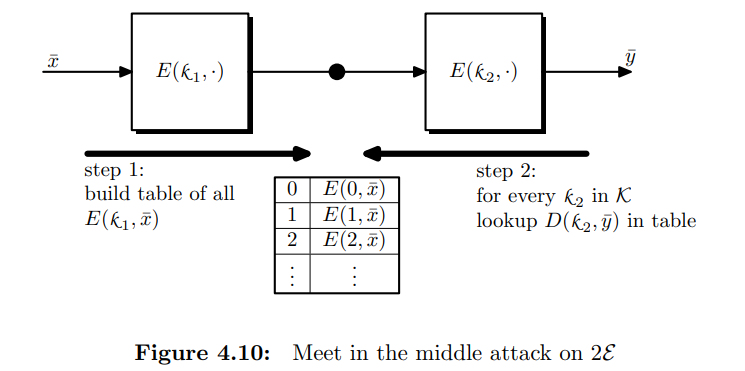
\includegraphics[width=0.8\textwidth]{Stanford_Crypto_1/fig/03_block_cipher/DES Meet in the Middle Attack.png}
    \caption{DES Meet in the Middle Attack}
    \label{fig: 03 DES Meet in the Middle Attack}
\end{figure}

\subsubsection{DESX}

Another method is DESX.

\begin{method} [DESX] DESX: 

    \begin{equation}
        \begin{aligned}
            &\mathrm{E}: \mathrm{K} \times\{0,1\}^{\mathrm{n}} \longrightarrow\{0,1\}^{\mathrm{n}} \text { a block cipher } \\
            &\text { Define } E X \text { as } \operatorname{EX}\left(\left(\mathrm{k}_{1}, \mathrm{k}_{2}, \mathrm{k}_{3}\right), \mathrm{m}\right)=\mathrm{k}_{1} \oplus \mathrm{E}\left(\mathrm{k}_{2}, \mathrm{~m} \oplus \mathrm{k}_{3}\right) \\
            &\text { For DESX: } \text { key-len }=64+56+64=184 \text { bits } \\
        \end{aligned}
    \end{equation}
    
\end{method}

DESX has an easy attack in time $2^{64+56}=2^{120}$ compared to its key length


\subsection{AES}

The high level overview of AES is shown in Figure \ref{fig: 03 AES High-level}. It is a substitution-permutation network.

\begin{figure}[h]
    \centering
    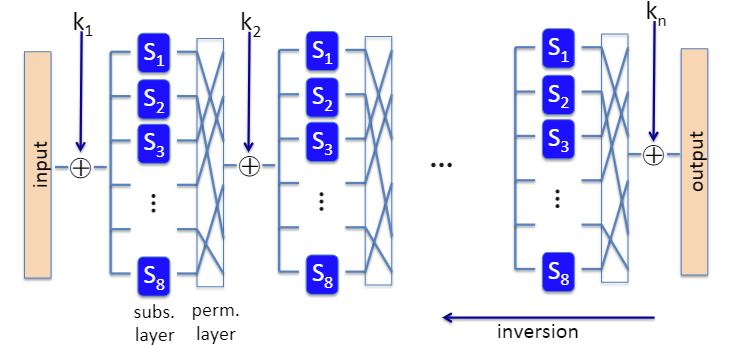
\includegraphics[width=0.8\textwidth]{Stanford_Crypto_1/fig/03_block_cipher/AES High-level.png}
    \caption{AES High-level}
    \label{fig: 03 AES High-level}
\end{figure}


\subsubsection{Schematic of AES-128}

The schematic of AES-128 is shown in Figure \ref{fig: 03 AES128 Schematic}.

\begin{figure}[h]
    \centering
    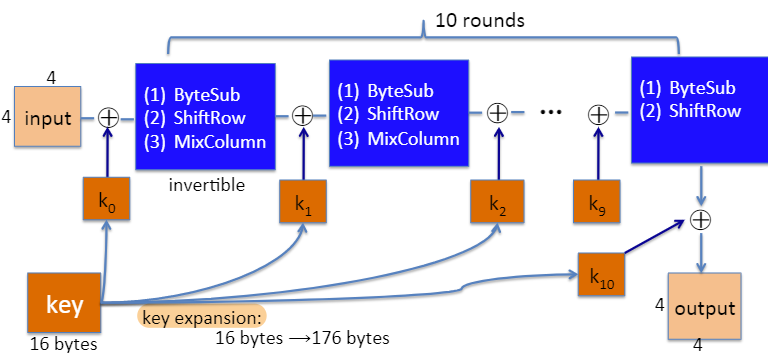
\includegraphics[width=0.8\textwidth]{Stanford_Crypto_1/fig/03_block_cipher/AES128 Schematic.png}
    \caption{AES128 Schematic}
    \label{fig: 03 AES128 Schematic}
\end{figure}

The auxiliary functions of AES is shown as follows:

\begin{enumerate}
    \item ByteSub: $A[i, 7]) \in S[A(i, J)]$
    \item ShiftRows: shown in Figure \ref{fig: 03 AES Auxialiary Functions}.
    \item MixColumns: shown in Fiugre \ref{fig: 03 AES Auxialiary Functions}
\end{enumerate}

\begin{figure}[h]
    \subfigure[ShiftRows]{
        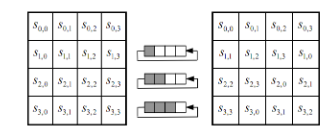
\includegraphics[width=0.5\textwidth]{Stanford_Crypto_1/fig/03_block_cipher/AES Shift Rows.png}
    }
    \subfigure[Mix Columns]{
        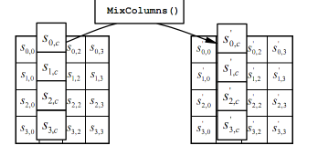
\includegraphics[width=0.5\textwidth]{Stanford_Crypto_1/fig/03_block_cipher/AES Mix Columns.png}
    }
    \caption{AES Auxialiary Functions}
    \label{fig: 03 AES Auxialiary Functions}
    
\end{figure}


\section{Security of Block Ciphers}

\subsection{Exhaustive Search Attacks}

The goal of exhaustive search attack is: given a few input output pairs $(m_i,c_i=E(k,m_i))$, find key.


\subsection{Semantic Security for Many-Time Key}

For the many-time key cases, the adversary is able to see many CTs with same key.

\begin{definition} [Chosen-Plaintext Attack(CPA)] Chosen-Plaintext Attack(CPA)

    The adversary is able to obtain the encryption of arbitrary messages of his choice.
    
\end{definition}

The attack game of many-time key is shown in Figure \ref{fig: 03 Attack of Sem Secure for Many-Time Key}.

\begin{figure}[h]
    \centering
    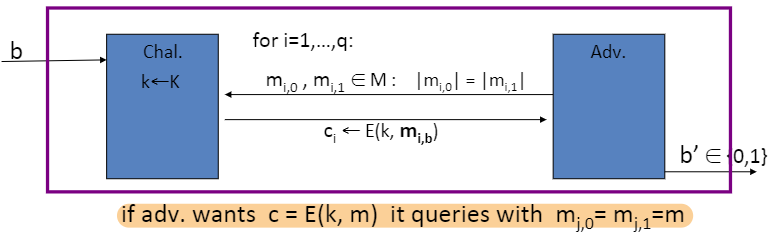
\includegraphics[width=0.8\textwidth]{Stanford_Crypto_1/fig/03_block_cipher/Attack of Sem Secure for Many-Time Key.png}
    \caption{Attack of Sem Secure for Many-Time Key}
    \label{fig: 03 Attack of Sem Secure for Many-Time Key}
\end{figure}

\begin{definition} [Sem. Sec with CPA]

    E is sem. sec. under CPA if for all "efficient" A:
    $$
    \operatorname{Adv}_{\text {CPA }}[A, E]=|\operatorname{Pr}[\operatorname{EXP}(0)=1]-\operatorname{Pr}[\operatorname{EXP}(1)=1]|
    $$
    is "negligible."
    
\end{definition}

If a system is not Sem. Sec. with CPA, this means an attacker can learn that two encrypted files are the same or two encrypted packets are the same. This is malicious, because like in a voice stream, the attacker will know the break time.

\subsubsection{Property}

Suppose $E(k,m)$ always outputs the same ciphertext for msg m, then it will not be secure with CPA (shown in Figure \ref{fig: 03 Ciphers Insecure under CPA}).

\begin{figure}[h]
    \centering
    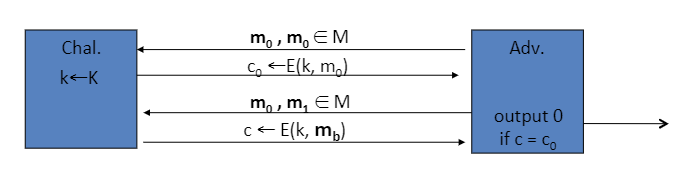
\includegraphics[width=0.8\textwidth]{Stanford_Crypto_1/fig/03_block_cipher/Ciphers Insecure under CPA.png}
    \caption{Ciphers Insecure under CPA}
    \label{fig: 03 Ciphers Insecure under CPA}
\end{figure}

This means, if a secret key is to be used multiple times, we should have: given the same plaintext message twice, the encryption must produce different outputs.

\subsubsection{Solution 1: Randomized Encryption}

The structure of the randomized encryption is shown in Figure \ref{fig: 03 Randomized Encrpytion}.

\begin{figure}[h]
    \centering
    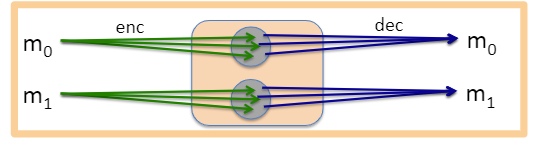
\includegraphics[width=0.8\textwidth]{Stanford_Crypto_1/fig/03_block_cipher/Randomized Encrpytion.png}
    \caption{Randomized Encryption}
    \label{fig: 03 Randomized Encrpytion}
\end{figure}

Which means we should use a $E(k,m)$ that is a randomized algorithm. However, it also means the ciphertext must be longer than plaintext. (because it is a one to n mapping)

\subsubsection{Solution 2: Nonce-Based Encryption}

\begin{definition} [nonce] nonce

    a value that changes from msg to msg.

    (k,n) pair never used more than once
    
\end{definition}

The structure of the nonce-based encryption is shown in Figure \ref{fig: 03 Nonce-Based Encryption}.


\begin{figure}[h]
    \centering
    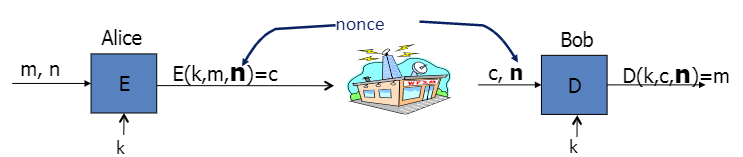
\includegraphics[width=0.8\textwidth]{Stanford_Crypto_1/fig/03_block_cipher/nonce-based encrpytion.png}
    \caption{Nonce-Based Encryption}
    \label{fig: 03 Nonce-Based Encryption}
\end{figure}

There are mainly two ways to define a nonce:
\begin{itemize} [itemsep=2pt,topsep=0pt,parsep=0pt]
    \item nonce is a counter, this is used when encryptor keeps state from msg to msg
    \item encryptor chooses a random nonce
\end{itemize}

The attack of nonce-based encryption is shown in Figure \ref{fig: 03 Attack for nonce-based encryption}.

\begin{figure}[h]
    \centering
    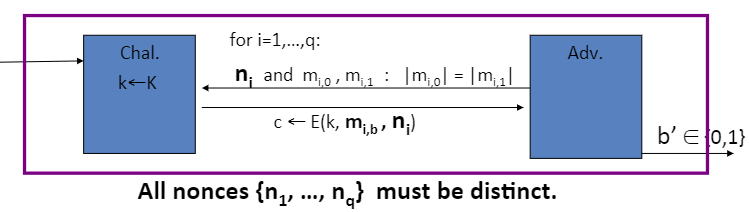
\includegraphics[width=0.8\textwidth]{Stanford_Crypto_1/fig/03_block_cipher/Attack for nonce-based encryption.png}
    \caption{Attack for nonce-based encryption}
    \label{fig: 03 Attack for nonce-based encryption}
\end{figure}

\begin{definition} [Sem.Secure for Nonce-Based E under CPA] Sem.Secure for Nonce-Based E under CPA:

    nonce-based $E$ is sem. sec. under CPA if for all "efficient" A:
    $\operatorname{Adv}_{\text {nCPA }}[A, E]=|\operatorname{Pr}[\operatorname{EXP}(0)=1]-\operatorname{Pr}[\operatorname{EXP}(1)=1]|$ is "negligible."
    
\end{definition}


\subsection{More Attacks on Block Ciphers}


\subsubsection{Attacks on the implementation}

There  are a lot of method to attack block cipher based on the implementation. So the main lesson is: \textbf{Don't Design Ciphers Yourself}



\subsection{Modes of Operations}

\subsection{ECB: An Incorrect Use of a PRP}


The electronic Code Block is a classical incorrect way of using a PRP. The structure of ECB is shown in Figure \ref{fig: 03 ECB Mode}.


\begin{figure}[h]
    \centering
    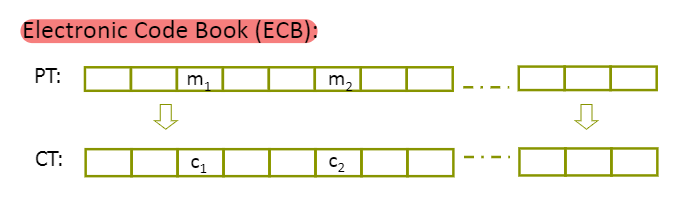
\includegraphics[width=0.8\textwidth]{Stanford_Crypto_1/fig/03_block_cipher/ECB Mode.png}
    \caption{ECB Mode}
    \label{fig: 03 ECB Mode}
\end{figure}


The problem of ECB is for the same message $m_1=m_2$ it will produce the same ciphertext $c_1=c_2$. So it will lost the CPA Attack.



\subsection{CBC with random IV}

CBC: Cipher Block Chain

IV: Initial Vector

The encrpytion and decryption process of CBC with random IV is shown in Figure \ref{fig: 03 CBC with random IV}.

\begin{figure}[h]
    \subfigure[Encryption]{
        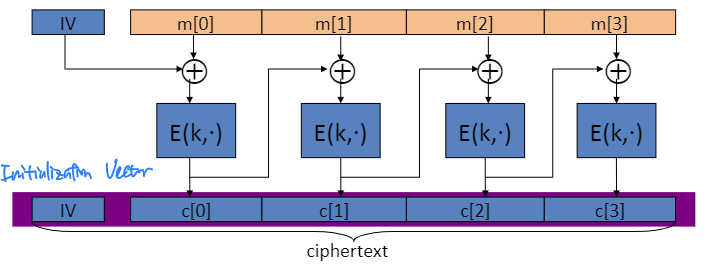
\includegraphics[width=0.5\textwidth]{Stanford_Crypto_1/fig/03_block_cipher/CBC with Random IV Encry.png}
    }
    \subfigure[Decyprtion]{
        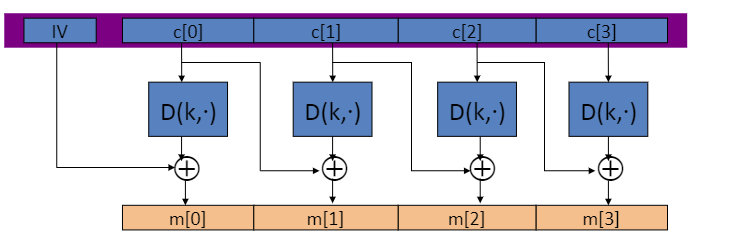
\includegraphics[width=0.5\textwidth]{Stanford_Crypto_1/fig/03_block_cipher/CBC with Random IV Decry.png}
    }
    \caption{CBC with random IV}
    \label{fig: 03 CBC with random IV}
\end{figure}

\subsubsection{Nonce-Based CBC}

The nonce-based CBC use a key pair $key=(k,k_1)$. It is a CBC with unique nonce, i.e. (key,n) pair is used for only one message. The structure of the nonce-based CBC is shown in Figure \ref{fig: 03 nonce-based CBC}.

\begin{figure}[h]
    \centering
    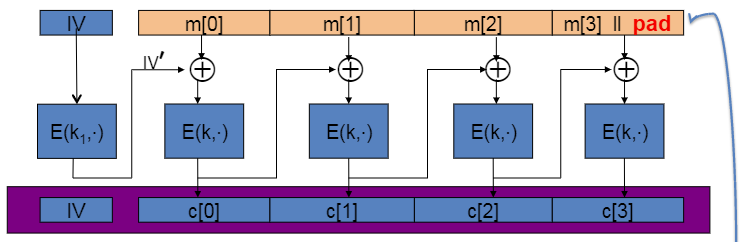
\includegraphics[width=0.8\textwidth]{Stanford_Crypto_1/fig/03_block_cipher/nonc-based CBC.png}
    \caption{Nonce-based CBC}
    \label{fig: 03 nonce-based CBC}
\end{figure}

\subsubsection{Padding in CBC}

The CBC mode need a padding part to extend the message in order to let the length becomes a multiple of block size. The pad is removed during decryption.

One example is the padding used in the TLS: for $n>0, n$ byte pad is \begin{tabular}{|l|l|l|l|l|} \hline$n$ & $n$ & $n$ & $\cdots$ & $n$ \\ \hline \end{tabular}
if no pad needed, add a dummy block


\subsubsection{CPA Security}

\begin{theorem} [CBC CPA Security]
    For any $L>0$,
    If $E$ is a secure PRP over $(K, X)$ then
    $E_{C B C}$ is a sem. sec. under $C P A$ over $\left(K, X^{L}, X^{L+1}\right)$.
    In particular, for a q-query adversary $A$ attacking $E_{C B C}$ there exists a PRP adversary B s.t.:
    $\operatorname{Adv}_{\mathrm{CPA}}\left[A, E_{\mathrm{CBC}}\right] \leq 2 \cdot \operatorname{Adv}_{\mathrm{PRP}}[B, E]+2 q^{2} L^{2} /|X|$
\end{theorem}

Based on the theorem, we know that after $w^{48}$ AES blocks, we must change key.

\textbf{Notes: } CBC where attacker can predict the IV is not CPA-secure.



\subsection{Random Counter(ctr) Mode}

Let $\mathrm{F}: \mathrm{K} \times\{0,1\}^{\mathrm{n}} \rightarrow\{0,1\}^{\mathrm{n}}$ be a secure PRF.
$\mathrm{E}(\mathrm{k}, \mathrm{m}):$ choose a random $\mathrm{IV} \in\{0,1\}^{\mathrm{n}}$.

Then the structure of the rand ctr-mode is shown in the Figure \ref{fig: 03 rand ctr-mode}.

\begin{figure}[h]
    \centering
    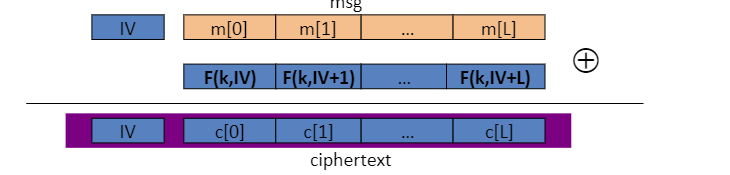
\includegraphics[width=0.8\textwidth]{Stanford_Crypto_1/fig/03_block_cipher/rand ctr-mode.png}
    \caption{rand ctr-mode}
    \label{fig: 03 rand ctr-mode}
\end{figure}

This is a \textbf{parallelizable structure}

\subsubsection{Nonce-Based ctr mode}


\subsubsection{CPA Security}

\begin{theorem} [CPA Security for CTR Mode] CPA Security for CTR Mode:

    Counter-mode Theorem: For any $L>0$,
    If $F$ is a secure PRF over $(K, X, X)$ then
    $E_{C T R}$ is a sem. sec. under CPA over $\left(K, X^{L}, X^{L+1}\right)$.
    In particular, for a q-query adversary $A$ attacking $E_{C T R}$
    there exists a PRF adversary B s.t.:
    $\operatorname{Adv}_{\mathrm{CPA}}\left[A, E_{\mathrm{CTR}}\right] \leq 2 \cdot \operatorname{Adv}_{\mathrm{PRF}}[B, F]+2 q^{2} L /|X|$
    
\end{theorem}

ctr-mode only secure as long as $q^{2} L<|X|$. Better than $C B C$. Based on the theorem, if we use AES in CTR mode, after $2^32$ CTs each of len $2^32$, we must change key. 

\section{Summary}
This chapter, we start from PRP and PRF. We defined what is secure PRF and secure PRP. And we propose method to construct PRF or PRG from each other. 

Then we introduce two useful method of block cipher: AES and DES. AES is much more safer while DES is less safer and we always use 3-DES.

Then we define the model of CPA Sem. Sec. Based on the CPA Sem. Sec., we knows that if we want to use the same key many times and keep safe, we need to let the same message generate different ciphertext. Based on that, we need the randomized algorithm or nonce-based algorithm. Which means we need to use PRG or PRF.

Besides, although we use some randomized component, how to use it is also a big problem. We knows that ECB is not secure. Classical secure modes of operation contains: CBC mode and CTR mode.

\chapter{Integrity}

\section{Message Integrity}

The goal of message integrity is integrity, that is, the information must be protected against any malicious modification.

\subsection{MACs}

\subsubsection{MAC Framework}

\begin{definition}[MAC] MAC:

    MAC I=(S,V) defined over (K,M,T) is a pair of algorithms:
    \begin{itemize} [itemsep=2pt,topsep=0pt,parsep=0pt]
        \item Signing Function: S(k,m) outputs a tag t in time T
        \item Verification Function: V(k,m,t) outputs 'yes' or 'no'
    \end{itemize}
    
\end{definition}

The basic framework of MAC is shown in Figure \ref{fig: Lecture 4: MAC FrameWork}.

\begin{figure}[h]
    \centering
    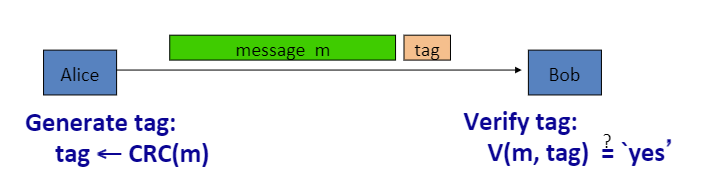
\includegraphics[width=0.8\textwidth]{Stanford_Crypto_1/fig/04_Integrity/MAC Frame Work.png}
    \caption{MAC FrameWork}
    \label{fig: Lecture 4: MAC FrameWork}
\end{figure}


\subsection{Secure MAC}

\subsubsection{Attackers in MACs}

Attacker's Power: chosen message attack, that is attacker can given $m_1, m_2, \cdots, m_q$, and an oracle will give back $\mathrm{t}_{\mathrm{i}} \leftarrow \mathrm{s}\left(\mathrm{k}, \mathrm{m}_{\mathrm{i}}\right)$.

Attacker's Goal: existential forgery, that is to produce some new valid message/tag pair (m,t), $(\mathrm{m}, \mathrm{t}) \notin\left\{\left(\mathrm{m}_{1}, \mathrm{t}_{1}\right), \ldots,\left(\mathrm{m}_{\mathrm{q}}, \mathrm{t}_{\mathrm{q}}\right)\right\}$.


\subsubsection{Motivation of Secure MAC}

intuitively, we have two expectations, A secure MAC should be able to:
\begin{enumerate} [itemsep=2pt,topsep=0pt,parsep=0pt]
    \item an attacker cannot produce a valid tag for a new message,  even for a gibberish message
    \item given (m,t), attacker cannot even produce (m,t') for $t' \neq t$
\end{enumerate}

\subsubsection{Definition of Secure MAC}

A game in MAC is defined as in Figure \ref{fig: Lecture 4: Game for MAC}.

\begin{figure}[h]
    \centering
    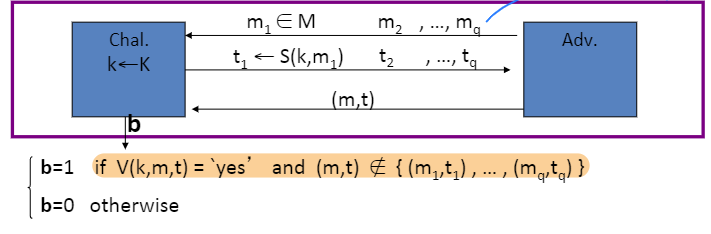
\includegraphics[width=0.8\textwidth]{Stanford_Crypto_1/fig/04_Integrity/Game for MAC.png}
    \caption{Game for MAC}
    \label{fig: Lecture 4: Game for MAC}
\end{figure}

One thing should be notice that, here, the adversary actually do not know the Ciphertext.

So we can generate the following definition of \textbf{secure MAC}
 
\begin{definition} [Secure MAC] Secure MAC

    I=(S,V) is a \textbf{secure MAC} if for  all "efficient" A, 
    $$
    \operatorname{Adv}_{\mathrm{MAC}}[A, I]=\operatorname{Pr}[\text { Chal. outputs } 1] \quad \text { is "negligible." }
    $$
\end{definition}


\section{Collision Resistance}

\subsection{Introduction}

Here are the definitions of \textbf{collision} and \textbf{collision resistant}.

\begin{definition} [collision and collision resistant] collision and collision resistant:

    Let $H: M \rightarrow T$ be a hash function $\quad(|M|>>|T|)$
    A collision for $\mathrm{H}$ is a pair $\mathrm{m}_{0}, \mathrm{~m}_{1} \in \mathrm{M}$ such that:
    $$
    \mathrm{H}\left(\mathrm{m}_{0}\right)=\mathrm{H}\left(\mathrm{m}_{1}\right) \text { and } \mathrm{m}_{0} \neq \mathrm{m}_{1}
    $$
    A function $\mathrm{H}$ is collision resistant if for all (explicit) "eff" algs. A:
    $\operatorname{Adv}_{\mathrm{CR}}[\mathrm{A}, \mathrm{H}]=\operatorname{Pr}[\mathrm{A}$ outputs collision for $\mathrm{H}]$
    is "neg".
    
\end{definition}

\subsection{Generic Birthday Attack}

\subsubsection{Generic Attack on C.R. functions}

\begin{method} [Generic Attack] Generic Attack:

\begin{enumerate} [itemsep=2pt,topsep=0pt,parsep=0pt]
    \item Choose $2^{n / 2}$ random messages in $M$ : $m_{1}, \ldots, m_{2}^{n / 2} \quad$ (distinct w.h.p)
    \item For $\mathrm{i}=1, \ldots, 2^{\mathrm{n} / 2}$ compute $\mathrm{t}_{\mathrm{i}}=\mathrm{H}\left(\mathrm{m}_{\mathrm{i}}\right) \quad \in\{0,1\}^{\mathrm{n}}$
    \item Look for a collision $\left(t_{i}=t_{j}\right)$. If not found, got back to step 1 .
\end{enumerate}

\end{method}

The time complexity of this method is $\mathcal{O}(2^{n/2})$

\subsubsection{The Birthday Paradox}

\begin{theorem} [The Birthday Paradox] The Birthday Paradox:

    when $\mathrm{n}=1.2 \times \mathrm{B}^{1 / 2}$ then $\operatorname{Pr}\left[\exists \mathrm{i} \neq \mathrm{j}: \mathrm{r}_{\mathrm{i}}=\mathrm{r}_{\mathrm{j}}\right] \geq 1 / 2$
\end{theorem}

\textbf{Notes:} If the distribution is uniform distribution, than it is the best case. Other distribution will lead to worse case.

The birthday paradox is illustrated in Figure \ref{fig: Lecture 4: The Birthday Paradox}.

\begin{figure}[h]
    \centering
    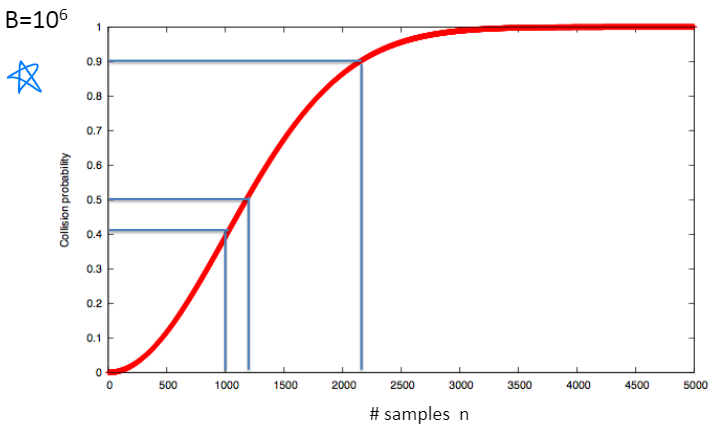
\includegraphics[width=0.8\textwidth]{Stanford_Crypto_1/fig/04_Integrity/The birthday paradox.png}
    \caption{The Birthday Paradox}
    \label{fig: Lecture 4: The Birthday Paradox}
\end{figure}

Based on the birthday paradox, if we use the generic attack, the expected number of iteration is roughly equal to 2.

\section{Construction of Collision Resistance}

The construction will be divided into two steps:

\begin{enumerate} [itemsep=2pt,topsep=0pt,parsep=0pt]
    \item given C.R. function for short messages, we can construct C.R. function for long messages. (The Merkle-Damagard Paradigm). That is, if we can find a C.R. compression function, then we can build a C.R. Hash function.
    \item Then we will propose some method to build C.R. compression function
\end{enumerate}

\subsection{The Merkle-Damagard Paradigm}

The structure of the Merkle-Damagard Paradigm is shown in Figure \ref{fig: Lecture 4: MD Framework}.

\begin{figure}[h]
    \centering
    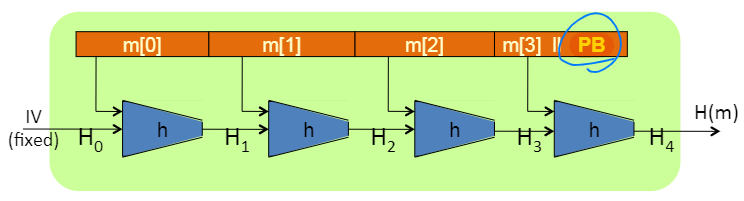
\includegraphics[width=0.8\textwidth]{Stanford_Crypto_1/fig/04_Integrity/MD iterated construction.png}
    \caption{MD Framework}
    \label{fig: Lecture 4: MD Framework}
\end{figure}

That is given $\mathrm{h}: \mathrm{T} \times \mathrm{X} \rightarrow \mathrm{T} \quad$ (compression function), we obtain $\mathrm{H}: \mathrm{X}^{\leq \mathrm{L}} \longrightarrow \mathrm{T} . \quad$ ($\mathrm{H}_{\mathrm{i}}-$chaining variables).

The \textbf{PB} part is the padding block. [10000$\cdots$000 || msg\_len(64-bits)]. If no space for PB, then add another block.

Based on Merkle-Damagard Paradigm, we have a theorem

\begin{theorem} [MD Collision Resistance] MD Collision Resistance:

    If h is C.R., then so is H
    
\end{theorem}

The proof is quite simple from final part and rollback.

\textbf{Notes: } The MD C.R. theorem told us, if we want to construct C.R. function, suffices to construct compression function.


\subsection{Constructing Compression Functions}

\subsubsection{Construct Compression Function from Block Cipher}

One method called \textbf{Davies-Meyer} Method: $\mathrm{h}(\mathrm{H}, \mathrm{m})=\mathrm{E}(\mathrm{m}, \mathrm{H}) \oplus \mathrm{H}$  and is shown in Figure \ref{fig: Lecture 4: Davies_Meyer Method}.

\begin{figure}[h]
    \centering
    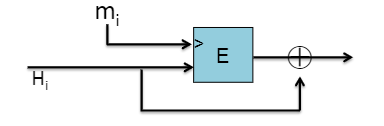
\includegraphics[width=0.5\textwidth]{Stanford_Crypto_1/fig/04_Integrity/Davies_Meyer Method.png}
    \caption{Davies\_Meyer Method}
    \label{fig: Lecture 4: Davies_Meyer Method}
\end{figure}

\begin{theorem}
    Suppose $E$ is an ideal cipher (collection of $|K|$ random perms.). Finding a collision $\mathrm{h}(\mathrm{H}, \mathrm{m})=\mathrm{h}\left(\mathrm{H}^{\prime}, \mathrm{m}^{\prime}\right)$ takes $\mathrm{O}\left(2^{n / 2}\right)$ evaluations of $(\mathrm{E}, \mathrm{D})$.
\end{theorem}

One application of the Davies-Meyer method is the SHA-256, which is shown in Figure \ref{fig: Lecture 4: SHA256 DM Method}.

\begin{figure}[h]
    \centering
    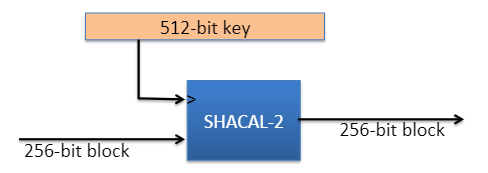
\includegraphics[width=0.5\textwidth]{Stanford_Crypto_1/fig/04_Integrity/SHA256 DM Method.png}
    \caption{SHA256 DM Method}
    \label{fig: Lecture 4: SHA256 DM Method}
\end{figure}


\subsubsection{Provable Compression functions}

\begin{method} [Provable Compression functions] Provable Compression functions: 

    Choose a random 2000-bit prime $p$ and random $1 \leq u, v \leq p$.
    For $m, h \in\{0, \ldots, p-1\} \quad$ define $\quad h(H, m)=u^{H} \cdot v^{m} \quad(\bmod p)$
\end{method}

\textbf{Fact: } finding collision for h is as hard as solving "discrete-log" module p. The problem of this method is that it is too slow.



\section{MACs based on PRFs}

\subsubsection{Property}

\begin{theorem} [From Secure PRF to Secure MAC] From Secure PRF to Secure MAC:

    If $\mathrm{F}: \mathrm{K} \times \mathrm{X} \rightarrow \mathrm{Y}$ is a secure PRF and $1 /|\mathrm{Y}|$ is negligible (i.e. $|Y|$ is large) then $I_{F}$ is a secure MAC.
    
    In particular, for every eff. MAC adversary A attacking $I_F$ there exists an eff. PRF adversary B attacking F s.t.:
    $$
    \operatorname{Adv}_{\mathrm{MAC}}\left[\mathrm{A}, \mathrm{I}_{F}\right] \leq \operatorname{Adv}_{\mathrm{PRF}}[\mathrm{B}, \mathrm{F}]+1 /|\mathrm{Y}|
    $$
    
\end{theorem}

\textbf{Notes: $I_F$ is secure as long as $|Y|$ is large}

And we can regard \textbf{AES} as a MAC for 16-byte messages.

\subsubsection{Motivation}

Given a PRF for short messages (AES), construct a PRF for long messages.


\subsection{ECBC-MAC}

The structure of ECBC-MAC is shown in Figure \ref{fig: Lecture 4: ECBC-MAC Structure}.

\begin{figure}[h]
    \centering
    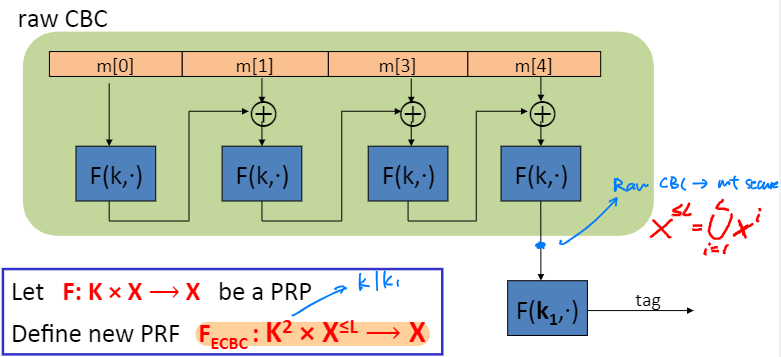
\includegraphics[width=0.8\textwidth]{Stanford_Crypto_1/fig/04_Integrity/CBC_MAC Structure.png}
    \caption{ECBC-MAC Structure}
    \label{fig: Lecture 4: ECBC-MAC Structure}
\end{figure}


One problem is Why the last Encryption step in ECBC-MAC?

Suppose we define a MAC $I_{\text {RAW }}=(S, V) \quad$ where
$$
S(k, m)=\operatorname{rawCBC}(k, m)
$$
Then $I_{\text {RAW }}$ is easily broken using a 1-chosen msg attack.

Adversary works as follows:
\begin{enumerate} [itemsep=2pt,topsep=0pt,parsep=0pt]
    \item choose an arbitrary one-block message $m \in X$
    \item request tag for m, Get $t=F(k,m)$
    \item Output t as MAC forgery for the 2-block message (m, t $\oplus$ m)
\end{enumerate}


Then the adversary win the challenge: $\operatorname{rawCBC}(k,(m, t \oplus m))=F(k, F(k, m) \oplus(t \oplus m))=F(k, t \oplus(t \oplus m))=t$

\subsubsection{CBC-MAC Padding}

For security, padding must be invertible, i.e.  $m_{0} \neq m_{1} \Rightarrow \quad \operatorname{pad}\left(m_{0}\right) \neq \operatorname{pad}\left(m_{1}\right)$.

The first method is the \textbf{ISO} standard: pad with "1000...00". Add new dummy block if needed. The " 1 " indicates beginning of pad. The structure of the ISO standard padding is shown in Figure \ref{fig: Lecture 4: ISO CBC Padding}.


\begin{figure}[h]
    \centering
    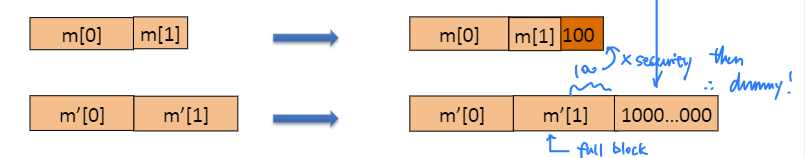
\includegraphics[width=0.8\textwidth]{Stanford_Crypto_1/fig/04_Integrity/ISO CBC Padding.png}
    \caption{ISO CBC Padding}
    \label{fig: Lecture 4: ISO CBC Padding}
\end{figure}


The second method is the \textbf{NIST} standard: it use a key tuple: $key=(k,k_1,k_2)$, in which, $(k_1,k_2)$ are derived from k. From this standard, we do not need the final encryption step of ECBC, and we do not need dummy block. The structure of the NIST standard padding is shown in Figure \ref{fig: Lecture 4: NIST CBC Padding}.

\begin{figure}[h]
    \centering
    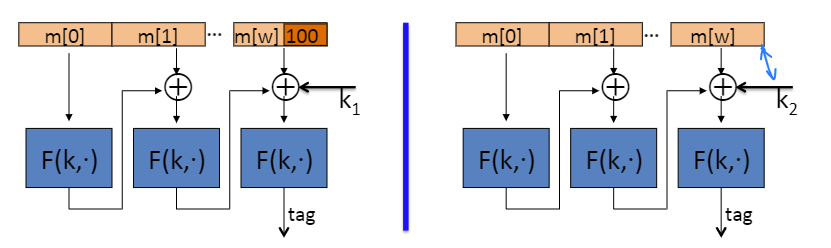
\includegraphics[width=0.8\textwidth]{Stanford_Crypto_1/fig/04_Integrity/NIST CBC Padding.png}
    \caption{NIST CBC Padding}
    \label{fig: Lecture 4: NIST CBC Padding}
\end{figure}

\subsubsection{Randomize MAC}

Another form of MAC with better security is shown in Figure \ref{fig: Lecture 4: Randomize MAC}

\begin{figure}[h]
    \centering
    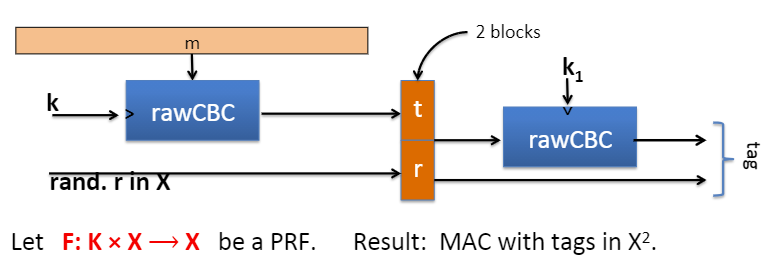
\includegraphics[width=0.8\textwidth]{Stanford_Crypto_1/fig/04_Integrity/Randomize MAC.png}
    \caption{Randomize MAC}
    \label{fig: Lecture 4: Randomize MAC}
\end{figure}

The security of this method is:  $A d v_{\mathrm{MAC}}\left[A, I_{\mathrm{RCBC}}\right] \leq A d v_{\mathrm{PRP}}[B, F] \cdot\left(1+2 q^{2} /|X|\right)$


\subsection{NMAC}

The structure of NMAC is shown in Figure \ref{fig: Lecture 4: NMAC Structure}.

\begin{figure}[h]
    \centering
    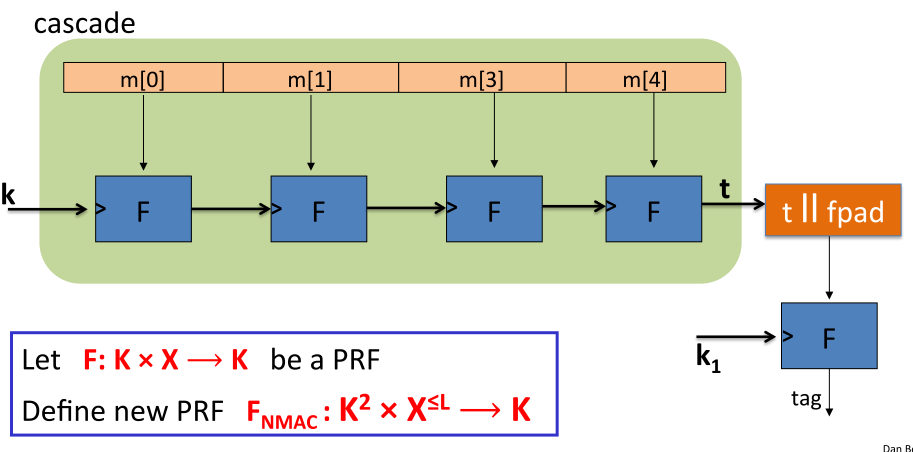
\includegraphics[width=0.8\textwidth]{Stanford_Crypto_1/fig/04_Integrity/NMAC Structure.png}
    \caption{NMAC Structure}
    \label{fig: Lecture 4: NMAC Structure}
\end{figure}

\subsection{Security Analysis of ECBC-MAC and NMAC}


\begin{theorem} [Security of ECBC-MAC and NMAC] Security of ECBC-MAC and NMAC:

    For any $L>0$,
    For every eff. q-query PRF adv. A attacking $F_{E C B C}$ or $F_{\text {NMAC }}$ there exists an eff. adversary B s.t.:
    $$
    \begin{aligned}
    &\operatorname{Adv}_{\mathrm{PRF}}\left[A, F_{\mathrm{ECBC}}\right] \leq \operatorname{Adv}_{\mathrm{PRP}}[B, F]+2 q^{2} /|X| \\
    &\operatorname{Adv}_{\mathrm{PRF}}\left[A, F_{\mathrm{NMAC}}\right] \leq q \cdot L \cdot \operatorname{Adv}_{\mathrm{PRF}}[B, F]+q^{2} / 2|K|
    \end{aligned}
    $$

\end{theorem}

\textbf{Notes:} CBC-MAC is secure as long as $q \ll<|X|^{1 / 2}$ NMAC is secure as long as $q<|K|^{1 / 2}$

An example using this theorem:

Suppose we want $\operatorname{Adv}_{\mathrm{PRF}}\left[\mathrm{A}, \mathrm{F}_{\mathrm{ECBC}}\right] \leq 1 / 2^{32} \Leftrightarrow \mathrm{q}^{2} /|\mathrm{X}|<1 / 2^{32}$
Then for AES: $|X|=2^{128} \Rightarrow q<2^{48}$
So, after $2^{48}$ messages must, must change key\

\subsubsection{Comparison of ECBC-MAC and NMAC}

ECBC-MAC is commonly used as an AES-based MAC.

NMAC not usually used with AES or 3DES. Main reason is: it need to change AES key on every block, requires re-computing AES key expansion.


\subsection{PMAC}

The structure of paralle MAC (PMAC) is shown in Figure \ref{fig: Lecture 4: PMAC Structure}

\begin{figure}[h]
    \centering
    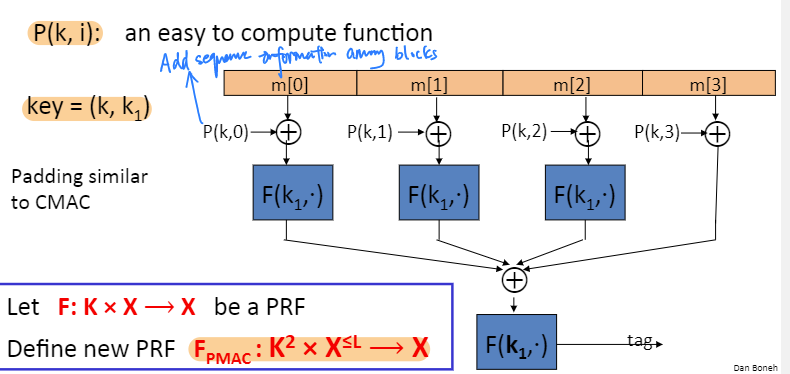
\includegraphics[width=0.8\textwidth]{Stanford_Crypto_1/fig/04_Integrity/PMAC_Structure.png}
    \caption{PMAC Structure}
    \label{fig: Lecture 4: PMAC Structure}
\end{figure}


\subsubsection{Property of PMAC}

PMAC is \textbf{incremental}. Which means we can easily generate a new tag when only one part of the PMAC is changed. For example when $m[1] \leftarrow m'[1]$, we can just do $\mathrm{F}^{-1}\left(\mathrm{k}_{1}, \mathrm{tag}\right) \oplus \mathrm{F}\left(\mathrm{k}_{1}, \mathrm{~m}[1] \oplus \mathrm{P}(\mathrm{k}, 1)\right) \oplus \mathrm{F}\left(\mathrm{k}_{1}, \mathrm{~m}^{\prime}[1] \oplus \mathrm{P}(\mathrm{k}, 1)\right)$


\subsubsection{Security Analysis}

\begin{theorem} [Security of PMAC] Security of PMAC:

    For any $L>0$,
    If $F$ is a secure PRF over $(K, X, X)$ then
    $F_{P M A C}$ is a secure PRF over $(K, X \leq L, X)$.
    For every eff. q-query PRF adv. A attacking $F_{\text {PMAC }}$ there exists an eff. PRF adversary B s.t.:
    $\operatorname{Adv}_{\mathrm{PRF}}\left[\mathrm{A}, \mathrm{F}_{\mathrm{PMAC}}\right] \leq \operatorname{Adv}_{\mathrm{PRF}}[\mathrm{B}, \mathrm{F}]+2 \mathrm{q}^{2} \mathrm{~L}^{2} /|\mathrm{X}|$
    
\end{theorem}


From the theorem, we knows that: PMAC is secure as long as $q L \ll|X|^{1 / 2}$.


\subsection{Carter-Wegman MAC}

\subsubsection{One-time MAC}



\section{MACs from Collision Resistance}

\subsection{HMAC}

The HMAC method need two dependent keys and an IV. The structure of HMAC is shown in Figure \ref{fig: Lecture 4: HMAC Structure}. It can be presented by:


$$
\quad S(k, m)=H(k \oplus o p a d \| H(k \oplus i p a d \| m))
$$

\begin{figure}[h]
    \centering
    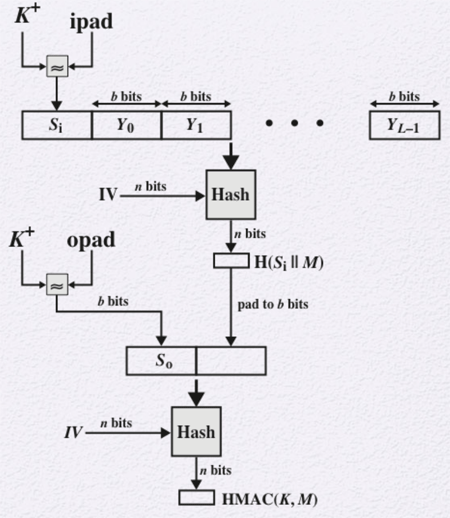
\includegraphics[width=0.5\textwidth]{Stanford_Crypto_1/fig/04_Integrity/HMAC Structure.png}
    \caption{HMAC Structure}
    \label{fig: Lecture 4: HMAC Structure}
\end{figure}

\subsubsection{Properties:}

HMAC is assumed to be a secure PRF
\begin{itemize} [itemsep=2pt,topsep=0pt,parsep=0pt]
    \item Can be proven under certain PRF assumptions about h(.,.)
    \item Security bounds similar to NMAC: Need $q^{2} /|T|$ to be negligible $\left(q<|T|^{1 / 2}\right)$
\end{itemize}

\section{Timing Attacks on MAC Verification}

Timing attacks try to use the step of Verification of the HMAC, because originally the earlier byte will be test first. So based on the feedback timing, some attacker try to find the real MAC.

So the lesson is \textbf{Don't implement crypto yourself}.


\section{Summary}
In this chapter, we first introduce what is an MAC, and we defined what is a secure MAC. The basic intuition is "the adversary cannot build a new (m,t) pair that is available".

Then we defined what is collision resistant and how to build collision resistant function from compression function and how to build compression function from Block Cipher. We also declared that we can regard AES as a PRF.

Then we illustrate three method for building MAC based on PRFs:  ECBC-MAC and NMAC and PMAC. And based on previous discussion of collision resistant function, we discussed the MAC based on collision resistant Hash Function: HMAC.


\chapter{Authenticated Encryption}



\section{Passive Attack and Active Attack}

The CPA Security can defend passive attack, however, it cannot defend active attack. In active attack, the attacker can not only get the plaintext, it can also get the ciphertext.

For example in Figure \ref{fig: 05 Example of Active Attack to MAC}. If the attacker get to know the ciphertext and message of the two message. It can easily generate a new (m,c,t) pair that is available. It can be done by just use $I V^{\prime}=I V \oplus(\ldots 80 \ldots) \oplus(\ldots . .25 \ldots)$.

\begin{figure}[h]
    \centering
    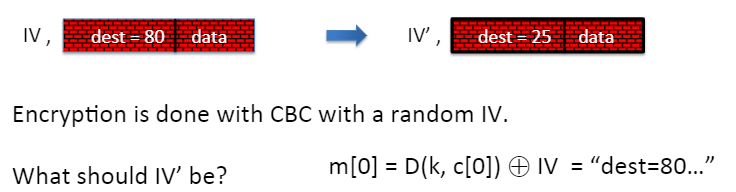
\includegraphics[width=0.5\textwidth]{Stanford_Crypto_1/fig/05_Authentication/An active attack to MAC.png}
    \caption{Example of Active Attack to MAC}
    \label{fig: 05 Example of Active Attack to MAC}
\end{figure}

So we have the conclusion that "CPA security cannot guarantee secret under active attacks". We should choose methods from:

\begin{enumerate}
    \item If message needs integrity but no confidentiality, use a MAC
    \item If message needs both integrity and confidentiality, use authenticated encryption modes
\end{enumerate}

\section{Chosen Ciphertext Attacks}

Adversary's power: both CPA and CCA
\begin{itemize}
    \item Can obtain the encryption of arbitrary message of his choice
    \item Can decrypt any ciphertext of his choice, other than challenge
\end{itemize}

The experiment about CCA is shown in Figure \ref{fig: 05 CCA Experiment}

\begin{figure}[h]
    \centering
    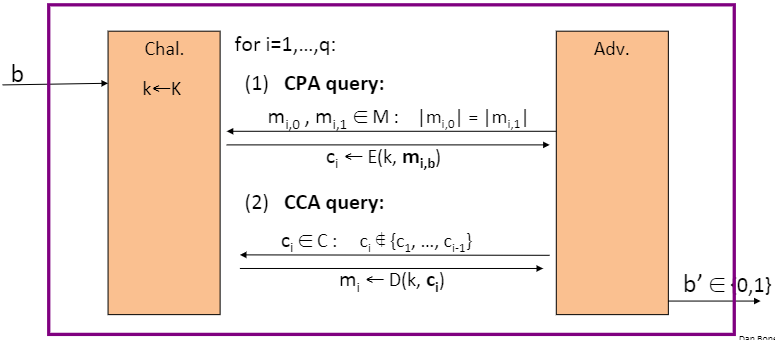
\includegraphics[width=0.5\textwidth]{Stanford_Crypto_1/fig/05_Authentication/CCA Experiment.png}
    \caption{CCA Experiment}
    \label{fig: 05 CCA Experiment}
\end{figure}

So we can define the security under CCA:

\begin{definition} [CCA Security]
    $\mathrm{E}$ is CCA secure if for all "efficient" A:
    $$
    \operatorname{Adv}_{C C A}[A, E]=|\operatorname{Pr}[\operatorname{EXP}(0)=1]-\operatorname{Pr}[\operatorname{EXP}(1)=1]| \text { is "negligible." }
    $$
    
\end{definition}

\section{Ciphetext Integrity}

The experiment for Ciphertext Integrity is shown in Figure \ref{fig: 05 Ciphertext Integrity}.

\begin{figure}[h]
    \centering
    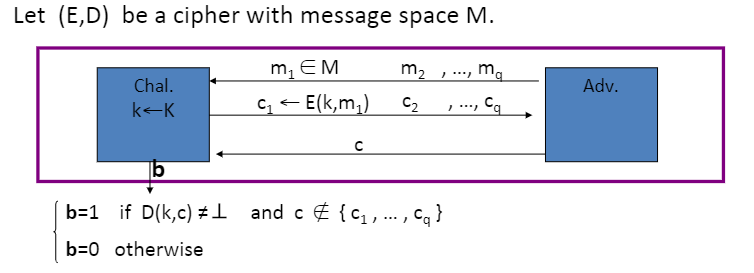
\includegraphics[width=0.5\textwidth]{Stanford_Crypto_1/fig/05_Authentication/Ciphertext Integrity.png}
    \caption{Ciphertext Integrity}
    \label{fig: 05 Ciphertext Integrity}
\end{figure}

Then we can define the Ciphertext Security:

\begin{definition} [Ciphertext Security] Ciphertext Security
    
    (E,D) has $\underline{\text { ciphertext integrity }}$ if for all "efficient" $A$ :
    $\operatorname{Adv}_{\mathrm{CI}}[A, E]=\operatorname{Pr}[$ Chal. outputs 1] $\quad$ is "negligible."
    
\end{definition}


\section{Authenticated Encryption}

\subsection{Conceptions}

\begin{definition}[Authenticated Encryption]  Authenticated Encryption
    
    An authenticated encryption system $(E, D)$ is a cipher where
    As usual:
    $\mathrm{E}: \mathrm{K} \times \mathrm{M} \times \mathrm{N} \rightarrow \mathrm{C}$
    but
    D: $K \times C \times N \rightarrow M \cup\{\perp\} \textbf{(which means the ciphertext is rejected)}$

\end{definition}

And we want the system provide:
\begin{itemize}
    \item Sem.Sec under a CPA attack
    \item Ciphertext integrity: attacker cannot create new ciphertexts that decrypt properly.
\end{itemize}


\begin{definition} [Authenticated Encryption Cipher] Authenticated Encryption Cipher:

    Cipher (E,D) provides authenticated encryption (AE) if it is:
    \begin{itemize}
        \item semantically secure under CPA, and
        \item has ciphertext integrity
    \end{itemize}
    
\end{definition}

A authenticated encryption cipher imply two things:
\begin{enumerate}
    \item Attacker cannot fool Bob into thinkging a message was sent from Alice: if $D(k, c) \neq \perp$ Bob knows message is from someone who knows $k$ (but message could be a replay)
    \item security against chosen ciphertext attack
\end{enumerate}


\subsection{Security Analysis}

\begin{theorem} [Authenticated Encryption and CCA Security] Authenticated Encryption and CCA Security

    Let $(E, D)$ be a cipher that provides $A E$.
    Then (E,D) is CCA secure!
    In particular, for any q-query eff. A there exist eff. B $_{1}, B_{2}$ s.t.
    $A d v_{C C A}[A, E] \leq 2 q \cdot A d v_{C C}\left[B_{1}, E\right]+A d v_{C P A}\left[B_{2}, E\right]$
        
\end{theorem}


\subsection{Constructions from Ciphers and MACs}

\subsubsection{MAC-then-Encrypt}

One example (SSL) of MAC-then-Encrypt  is shown in Figure \ref{fig: 05 MAC-then-Encrypt}. 


\begin{figure}[h]
    \centering
    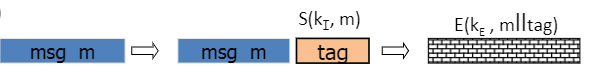
\includegraphics[width=0.5\textwidth]{Stanford_Crypto_1/fig/05_Authentication/M then E.png}
    \caption{MAC-then-Encrypt}
    \label{fig: 05 MAC-then-Encrypt}
\end{figure}


\subsubsection{Encrypt-then-MAC}

One example (IPsec) of Encrypt-then-MAC  is shown in Figure \ref{fig: 05 Encrypt-then-MAC}. 


\begin{figure}[h]
    \centering
    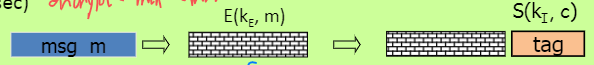
\includegraphics[width=0.5\textwidth]{Stanford_Crypto_1/fig/05_Authentication/E then M.png}
    \caption{Encrypt-then-MAC}
    \label{fig: 05 Encrypt-then-MAC}
\end{figure}


\subsubsection{Encrypt-and-MAC}

One example (SSH) of MAC-and-Encrypt  is shown in Figure \ref{fig: 05 Encrypt-and-MAC}.


\begin{figure}[h]
    \centering
    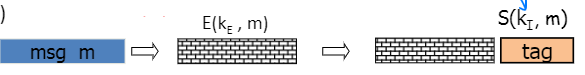
\includegraphics[width=0.5\textwidth]{Stanford_Crypto_1/fig/05_Authentication/E and M.png}
    \caption{Encrypt-and-MAC}
    \label{fig: 05 Encrypt-and-MAC}
\end{figure}


\subsubsection{Some Standard}

GCM, CCM, EAX.

All support AEAD (auth.enc.with associated data). All are nonce-based.

\subsection{Security Analysis}

Let (E,D) be CPA secure cipher and (S,V) secure MAC, then:

\begin{enumerate}
    \item Encrypt-then-MAC always provides A.E.
    \item MAC-then-Encrypt may be insecure against CCA attacks. However, wehn (E,D) is rand-CTR mode or rand-CBC, then it will be A.E.
\end{enumerate}

\subsection{Direct Construction from PRP: OCB}

The OCB frame work is shown in Figure \ref{fig: 05 OCB}.


\begin{figure}[h]
    \centering
    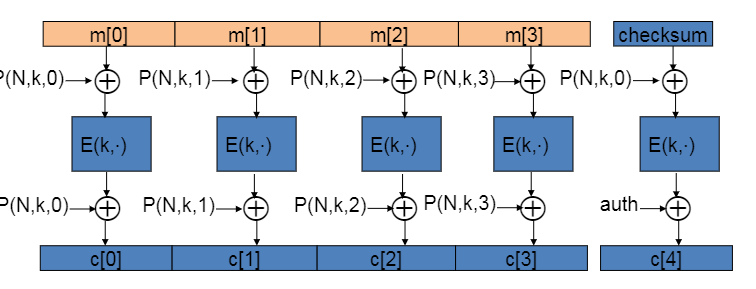
\includegraphics[width=0.5\textwidth]{Stanford_Crypto_1/fig/05_Authentication/OCB.png}
    \caption{OCB}
    \label{fig: 05 OCB}
\end{figure}


\subsection{CBC padding attacks}

Some lessons about CBC padding attacks:
\begin{itemize}
    \item Encrypt-then-MAC would completely avoid this problem
    \item MAC-then-CBC provides A.E., but padding oracle destroys it
\end{itemize}

\section{Summary}

Starting from the property of active attacker, we explained why the MAC cannot defend active attacker with an example. Then based on the fact that an active attacker can always see the ciphertext, we define the definition of ciphertext integrity and CCA Security.

Then we propose that Authenticated Encryption, that should be able to meet integrity and authenticated and be Sem. Sec under CCA. Then we introduce 3 ways to build an AE from MAC: E then M, M then E, M and E. And the fact is E then M always meet AE. Besides, we also mentioned one method to build an AE from PRP, the OCB method.

\chapter{Other Thing of Symmetric Encryption}
\section{Key Derivation}

\subsection{Motivation}

Typically, we can generate a single source key by:

\begin{enumerate}
    \item Hardware Random Number Generator
    \item A key exchange protocol
\end{enumerate}

However, based on previous contents, there are a lot of time that we need many keys for security. So the motivation of the Key Derivation is to generate many keys from this one source key.

\subsection{Case 1: Source Key is Uniform}

Suppose Source key SK is uniform in K. We can define key derivation function (KDF) as:

\begin{equation}
    \begin{aligned}
    &\text { KDF( SK, CTX, L) := } \\
    &\qquad F(S K,(C T X \| 0))\|F(S K,(C T X \| 1))\| \cdots \| F(S K,(C T X \| L))
    \end{aligned}
\end{equation}

where CTX is a string that uniquely identifies the application. The purpose of CTX is we want get independent keys even if two apps has sampled the same SK.

\subsection{Case 2: Source Key is not Uniform}

When SK is not uniform, the PRF output may not look random. And the fact is the source key often not uniformly random.

\subsubsection{Extract-then-Expand Paradigm}

The Extract-then-Expand Paradigm has two steps:

step 1: extract pseudo-random key k from source key SK, it is shown in Figure \ref{fig: 06 Extract-then-Expland Paradigm}. where \textbf{salt} is a fixed non-secret string chosen at random.

\begin{figure}[h]
    \centering
    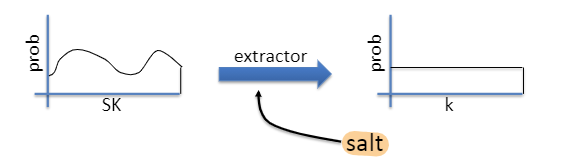
\includegraphics[width=0.5\textwidth]{Stanford_Crypto_1/fig/06_Other_Thing/Extract-then-Expland Paradigm.png}
    \caption{Extract-then-Expland Paradigm}
    \label{fig: 06 Extract-then-Expland Paradigm}
\end{figure}


step 2: expand k by using it as a PRF keys as before.


\subsubsection{HKDF: a KDF from HMAC}

Implements the extract-Then-expand paradigm:

Extract by: $\mathrm{k} \leftarrow HMAC( salt, SK)$ (salt is key, and SK is data)

Then expand using HMAC as a PRF with key $k$


\section{Deterministic Encryption}

Deterministic Encryption enables later lookup. However, attacker can tell when two ciphertexts encrypt the same message, which means we leak some information.

\subsection{Deterministic CPA Security}

The experiment of Deterministic CPA Security is shown in Figure \ref{fig: 06 Deterministic CPA Security}.

\begin{figure}[h]
    \centering
    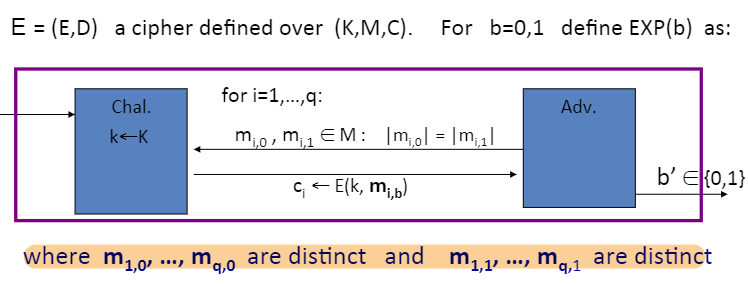
\includegraphics[width=0.5\textwidth]{Stanford_Crypto_1/fig/06_Other_Thing/Det CPA Security.png}
    \caption{Deterministic CPA Security}
    \label{fig: 06 Deterministic CPA Security}
\end{figure}

\begin{definition} [Sem Sec under det.CPA] em Sec under det.CPA

    $E$ is sem. sec. under det. CPA if for all efficient $A$ :
    $$
    \operatorname{Adv}_{\mathrm{dCPA}}[A, E]=|\operatorname{Pr}[\operatorname{EXP}(0)=1]-\operatorname{Pr}[\operatorname{EXP}(1)=1]| \quad \text { is negligible. }
    $$
    
\end{definition}

One should notice that: CBC with fixed IV is not det.CPA secure.


\section{Tweakable Encryption}



\section{Format Preserving Encryption}

\chapter{Basic Key Exchange}

\section{Trusted 3rd Parties}


\section{}


\subsection{Merkle Puzzles}


\subsection{The Diffie-Hellman Protocol}


\subsection{Public-Key Encryption}


\section{Modular Arithmetic}


\section{Easy and Hard Problems}

\end{document}